There are a number of buttons in the Push Button area of \Cref{fig:generic_ui}. This section describes the usage of these buttons.

\subsection{RUN}

This button allows the user to run the simulation on the local machine. When the button is 
pressed a window, as shown in \Cref{fig:run_button_popup}, will pop up informing the user 
that the UQ engine has started running. When complted this window will dissapear and the RES
panel will be selected.

NOTE: There are two input fields specified in the applications preferences that effects the running of the UQ engine. The typical user DOES NOT NEED TO MODIFY THE INFORMATION IN THE INPUT FIELDS. Advanced users can specify the locations of the following two directories here:

\begin{itemize}
\item Local Jobs Dir: specifies where the \texttt{\getsoftwarename{}} application shall
create a \texttt{tmp.SimCenter} directory for temporary files that are used to perform the simulation. This directory is created after the \texttt{Submit} button is pressed. As discussed in \Cref{chap:troubleshooting}, when
the application creates this directory it copies the files needed to it (e.g., if you are using OpenSees input script, it
will copy that script to the \texttt{tmp.SimCenter} directory. ALL FILES IN
THE SCRIPT DIRECTORY AND ALL FILES IN SUBDIRECTORIES OF THAT DIRECTORY GET
COPIED SO DON’T PLACE THE OPENSEES SCRIPT IN HOME, DOWNLOADS, DOCUMENTS, etc….
\item Local Application Dir: The \texttt{\getsoftwarename{}} application searches for the workflow applications in this directory. Only edit its location if you are introducing your own applications or you want to build and modify the 
applications provided with the tool. 
\end{itemize}

\subsection{RUN at DesignSafe}
This button when pressed will cause the UI to package the input information and send it to 
DesignSafe. At DesignSafe the inputs will be stored, a job will subsequently run on a 
supercomputer, and the results stored in the user's DesignSafe jobs folder. The simulation 
resucan be retrieved with the \texttt{GET from DesignSafe} button. After clicking on the 
button, the window shown in \Cref{fig:remote_button} pops up. There are several input fields 
and a \texttt{Submit} button in the window. 

\begin{figure}[!htbp]
  \centering {
    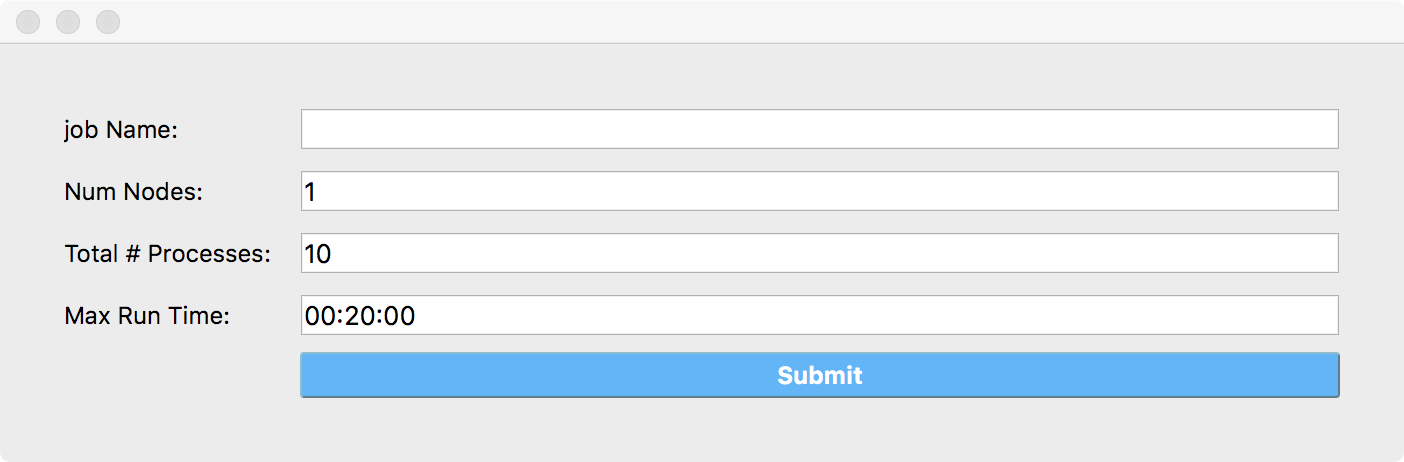
\includegraphics[width=0.8\textwidth]
    {usage/figures/remoteButton.png} }
  \caption{Pop-up window shown after clicking the \texttt{RUN at DesignSafe} button}
  \label{fig:remote_button}
\end{figure}

\begin{itemize}
\item Job Name: The name the user can use to identify the job in Get from DesignSafe.
\item Num Nodes: The number of compute nodes to use on Stampede2. Using the default App Name the job will run on Stampede2’s KNL Landing (KNL) 
compute nodes. Each node has 68 cores. The actual number of cores the
application will use on each of these nodes depends on the total
number of processes specified. As per the TACC webpage, for MPI tasks
it’s best not to specify more than 64-68 processes to run. Depending
on the numerical computations and amount of memory each uses, for large simulations you may wish to use more nodes and less processes to
avoid page faulting.
\item Total Number of Processes: Total number of MPI parallel processes the UQ engine is going to use.
\item Max Wall Time: Use HOURS:MIN:SEC format and be conservative. Your job is killed after the time limit is reached. On Stampede2 you have a max wall time of 24 hours.
\end{itemize}

Finally, when inputs are finished, the user presses the Submit button to start the process. If
the job gets submiitted successfully to DesignSafe the pop-up window will dissappear with a job successfully started message appearing in the message area. Do not press the Submit button multiple times, monitor the message area for progress. If the process appear stalled it may be due to a large number of requests being processed by DesignSafe. If this is the case it is sometimes best to close the popup, save the file, and try again later.

NOTE: Similar to running locally, there are additional options available in the preferences
 section that advanced users can modify that effect the running of the tool.
\begin{itemize}
\item Remote Jobs Directory: specifies where the \texttt{\getsoftwarename{}} application shall
create a \texttt{tmp.SimCenter} directory for temporary files that are used to perform the simulation. This directory is created after the \texttt{Submit} button is pressed. As discussed in \Cref{chap:troubleshooting}, when
the application creates this directory it copies the files needed to it (e.g., if you are using OpenSees input script, it
will copy that script to the \texttt{tmp.SimCenter} directory. ALL FILES IN
THE SCRIPT DIRECTORY AND ALL FILES IN SUBDIRECTORIES OF THAT DIRECTORY GET
COPIED SO DON’T PLACE THE OPENSEES SCRIPT IN HOME, DOWNLOADS, DOCUMENTS, etc…. The Working Directory is removed after the job has been submitted successfully.
\item Local Applications Directory: The \texttt{\getsoftwarename{}} application searches for the workflow applications in this directory. Only edit its location if you are introducing your own applications or you want to build and modify the 
applications provided with the tool. 
\item Remote Applications Directory: Remote directory on Stampede2 where applications needed by the workflow reside. Only modify if you have built the applications on the supercomputer, currently Stampede2.
\item App Name: Name of Agave app to run. Only modify you have created your own Agave app.
\end{itemize}

\subsection{GET from DesignSafe}
Allows you to obtain your list of jobs from DesignSafe and select from that list a job to update status of, download or delete.

\subsection{Exit}
Click this button to exit the application.
